\documentclass[12pt,a4paper,article,english,firamath]{nsi}
\pagestyle{empty}
\setfontfamily{\brettley}{Cursive standard}[Scale=1.5]
\begin{document}
\titre{Find your figure}
\classe{Euro 1\ere}
\maketitle

\subsection*{Description 3}
{\brettley 

Draw two perpendicular lines and a circle whose center is their intersection.
Choose one of this two lines. It has two points of intersection with the circle. By one of these points, draw a line parallel to the other. By the other one, draw a line passing through one intersection of the circle with the second line. This line intersects the parallel you drew before in a point which will be the center of a last circle, passing by the intersection of the first circle with the second line.}\\

\begin{tikzpicture}
    \draw[lightgray](0,0)--(\linewidth,0);
\end{tikzpicture}

\subsection*{Figure 3}
\begin{center}
    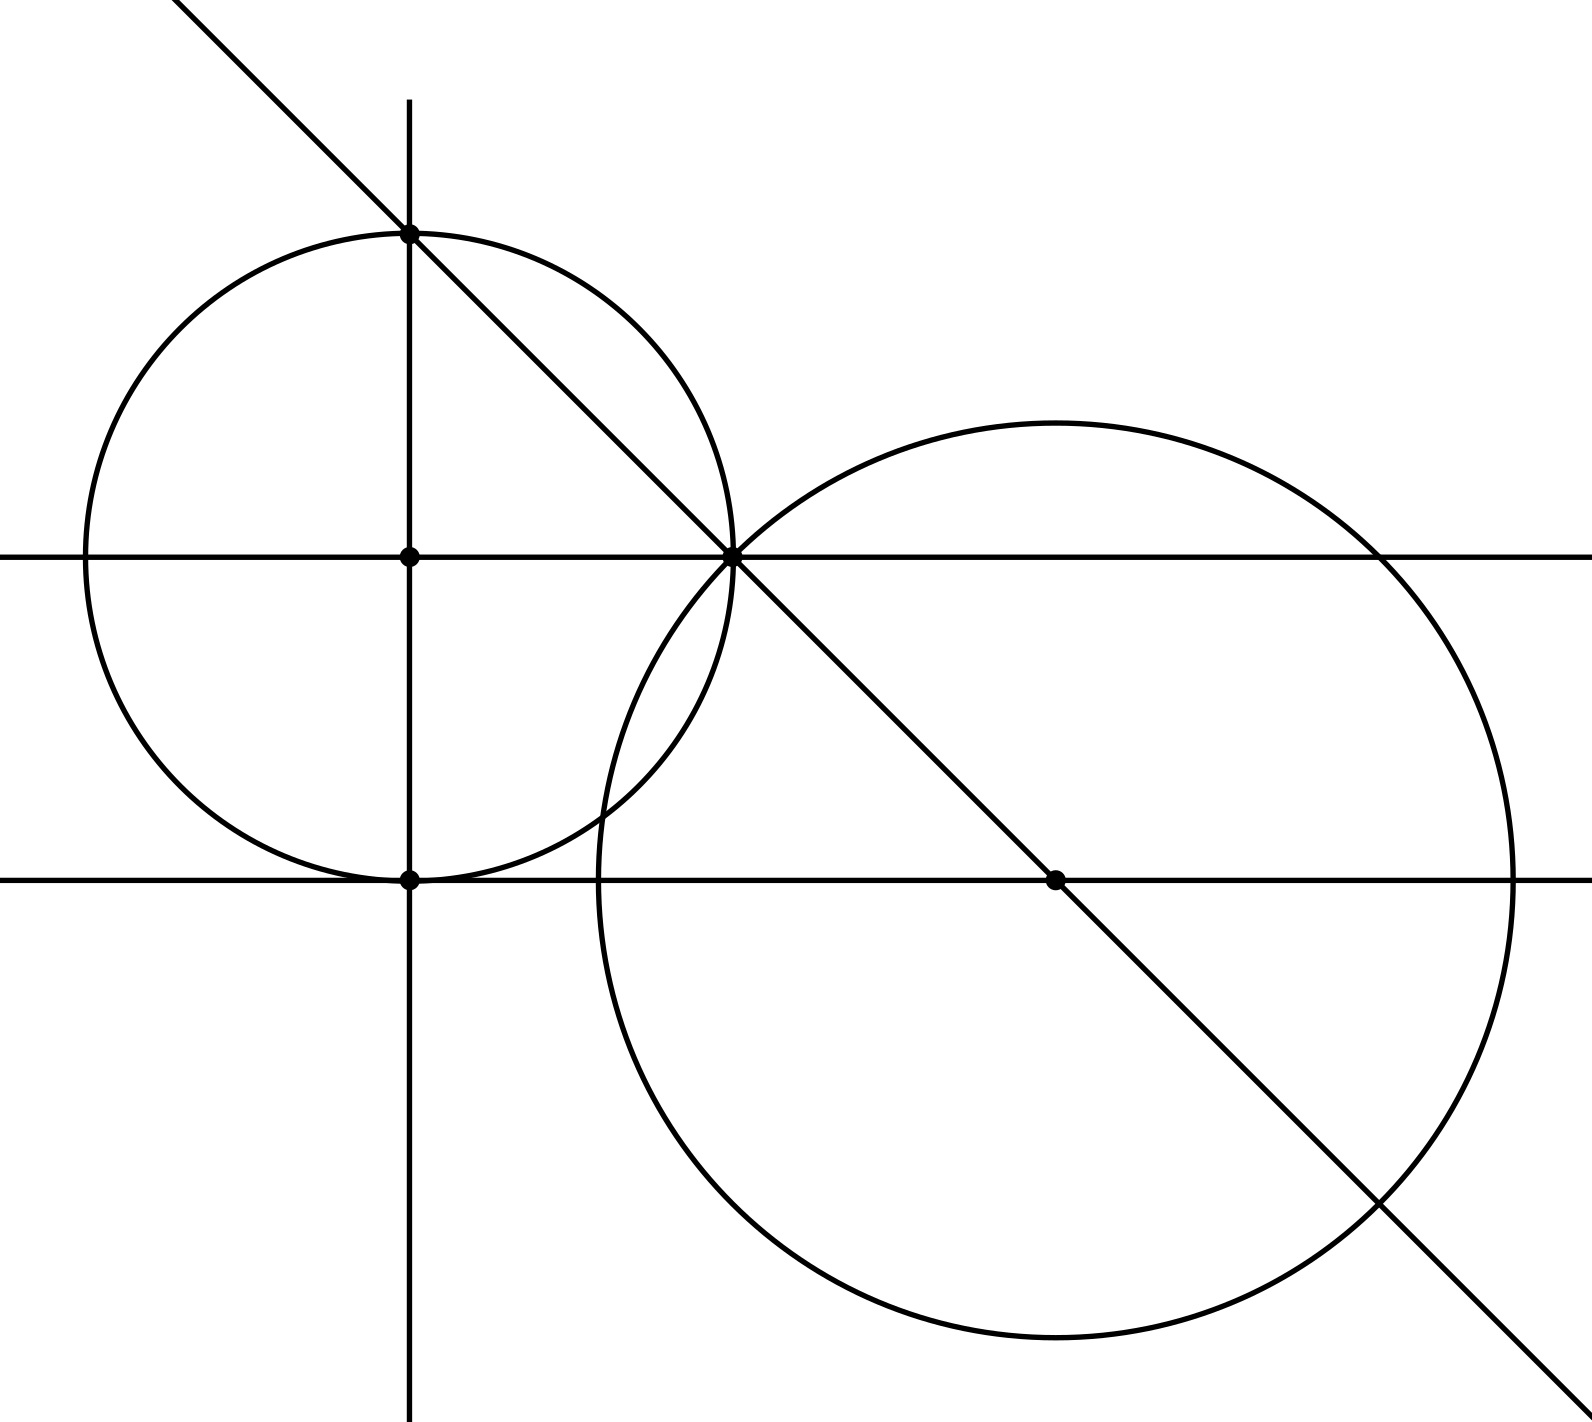
\includegraphics[height=11cm]{img/fig03.png}
\end{center}
\end{document}